% \begin{figure}[!ht]
% \centering
% 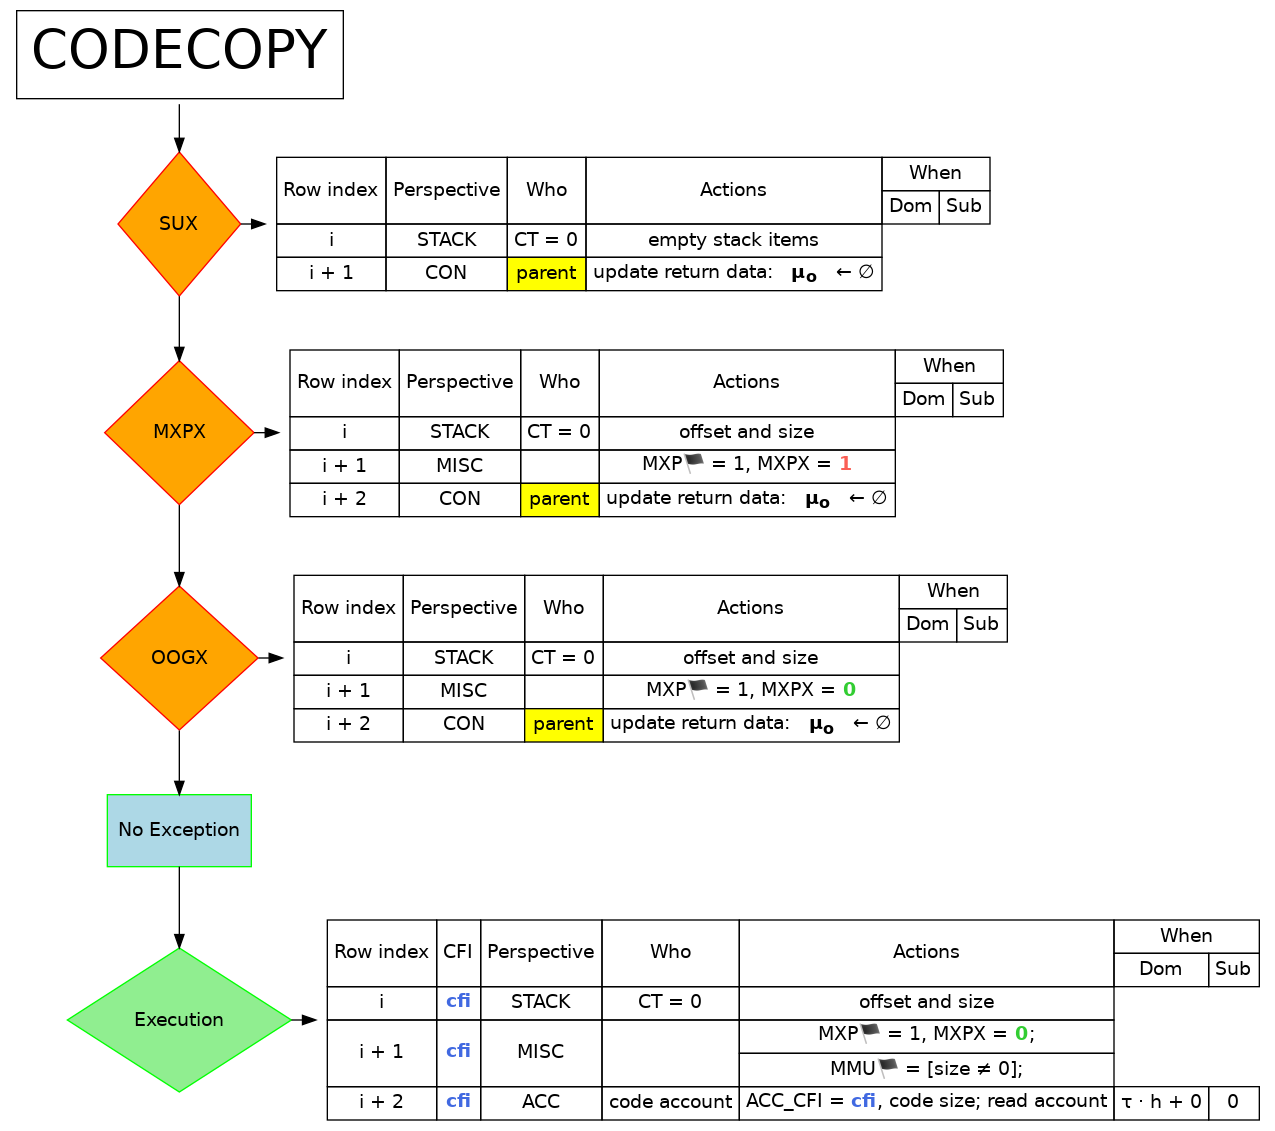
\includegraphics[width=\textwidth]{instruction_handling/copy/flowcharts/cc.png}
% 	\caption{General workflow for \inst{CODECOPY} instructions.}
% \label{fig: hub: instruction handling: copy: codecopy: general processing}
% \end{figure}

\begin{center}
	\boxed{%
		\text{The stack constraints presented below assume }
		\left\{ \begin{array}{lcl}
			\peekStack        _{i}                  & = & 1 \\
			\stackDecCopyFlag _{i}                  & = & 1 \\
			\locIsCc                                & = & 1 \\
			\stackSux         _{i} + \stackSox _{i} & = & 0 \\
		\end{array} \right.}
\end{center}
In other words we are dealing with a \inst{CODECOPY} instruction that doesn't raise a \suxSH{}.
Recall that this instruction either requires a context-row (if an exception occurs) or an account-row (otherwise.)
The specialized constraints are as follows:
\begin{description}
		% - [x] context stuff,
		% - [x] gas cost stuff,
		% - [∅] account stuff,
		% - [∅] trimming stuff,
		% - [∅] setting and unsetting warmth,
		% - [∅] account remain unchanged otherwise,
		% - [∅] etc ...
	\item[\underline{\underline{Setting the gas cost:}}]
		we only set the gas cost to the actual gas cost if no \mxpxSH{} has occurred (given no stack exception, that is):
		\begin{enumerate}
			\item \If $\stackMxpx _{i} = 1$ \Then $\gasCost_{i} = 0$
			\item \If $\stackOogx _{i} = 1$ \Then $\gasCost_{i} = \stackStaticGas_{i} + \locMxpGas$
			\item \If $\xAhoy     _{i} = 0$ \Then $\gasCost_{i} = \stackStaticGas_{i} + \locMxpGas$
		\end{enumerate}
		\saNote{} The above \emph{could} be subsumed under the single constraint
		\[
			\gasCost _{i} = (\stackOogx _{i} + (1 - \xAhoy _{i})) \cdot (\stackStaticGas_{i} + \locMxpGas) \quad (\trash)
		\]
	\item[\underline{\underline{Exceptional \inst{CODECOPY} case:}}]
		we impose that
		\begin{enumerate}
			\item \If $\xAhoy _{i} = 1$ \Then $\executionProvidesEmptyReturnData {i}{\locCopyCallerContextRowSmall} $ (\trash)
		\end{enumerate}
		\saNote{} Depending on whether the instruction produces an exception or not we either peek into the caller context (and provide it with empty return data) or inspect the current execution frame; we extract from it the following: call data offset, call data size and the datum of whether or not it is the root context.
	\item[\underline{\underline{Unexceptional \inst{CODECOPY} case:}}]
		\If $\xAhoy _{i} = 0$ \Then we impose
		\begin{description}
			\item[\underline{Setting the context row $n^°(i + \locCopyCurrentContextRow)$:}]
				we impose $\readContextData {i}{\locCopyCurrentContextRow}{\cn_{i}}$
			\item[\underline{Setting the account row $n^°(i + \locCopyCurrentAccountRow)$:}]
				we impose
				\[
					\left\{ \begin{array}{lclr}
						\accAddressHi          _{i + \locCopyCurrentAccountRow} & = & \cnCodeAddress\high _{i + \locCopyCurrentContextRow} \\
						\accAddressLo          _{i + \locCopyCurrentAccountRow} & = & \cnCodeAddress\low  _{i + \locCopyCurrentContextRow} \\
						\accDeploymentNumber   _{i + \locCopyCurrentAccountRow} & = & \relevantValue                                       \\
						\accDeploymentStatus   _{i + \locCopyCurrentAccountRow} & = & \relevantValue                                       \\
						\accCfi                _{i + \locCopyCurrentAccountRow} & = & \relevantValue                                       \\
						\accRomLexFlag         _{i + \locCopyCurrentAccountRow} & = & \nothing                                             \\
						\multicolumn{4}{l}{\accSameBalance                    {i}{\locCopyCurrentAccountRow}}    \\
						\multicolumn{4}{l}{\accSameNonce                      {i}{\locCopyCurrentAccountRow}}    \\
						\multicolumn{4}{l}{\accSameCode                       {i}{\locCopyCurrentAccountRow}}    \\
						\multicolumn{4}{l}{\accSameDeployment                 {i}{\locCopyCurrentAccountRow}}    \\
						\multicolumn{4}{l}{\accSameWarmth                     {i}{\locCopyCurrentAccountRow}}    \\
						\multicolumn{4}{l}{\accSameMarkedForSelfdestructFlag  {i}{\locCopyCurrentAccountRow}}    \\
						\multicolumn{4}{l}{
							\standardDomSubStamps {
								anchorRow        = i,
								relOffset        = \locCopyCurrentAccountRow,
								domOffset        = 0,
							}
						} \\
					\end{array} \right.
				\]
				\saNote{}
				The values of $\accDeploymentNumber _{i + \locCopyCurrentAccountRow}$ and $\accCfi _{i + \locCopyCurrentAccountRow}$ are implicitly constrained by account consistency constraints,
				see section~(\ref{hub: consistencies: account}).
				We may nonetheless include some ``sanity check'' constraints labeled by (\sanityCheck) to make the intent explicit:
				\[
					\left\{ \begin{array}{lcll}
						\accDeploymentNumber   _{i + \locCopyCurrentAccountRow} & = & \cnCodeDepNum       _{i + \locCopyCurrentContextRow} & (\sanityCheck)              \\
						\accDeploymentStatus   _{i + \locCopyCurrentAccountRow} & = & \cnCodeDepStatus    _{i + \locCopyCurrentContextRow} & (\sanityCheck)              \\
						\accCfi                _{i + \locCopyCurrentAccountRow} & = & \cnCodeCfi          _{i + \locCopyCurrentContextRow} & (\sanityCheck)              \\
						\accCfi                _{i + \locCopyCurrentAccountRow} & = & \cfi_{i}                                             & (\sanityCheck) \vspace{2mm} \\
						\accRomLexFlag         _{i + \locCopyCurrentAccountRow} & = & \rOne                                                & (\sanityCheck) ~ (\trash)   \\
					\end{array} \right.
				\]
				These constraints confront \textbf{account data} with \textbf{context data}.
				One constraint confronts \textbf{account data} with \textbf{shared data}.
				Note furthermore that turning on the \accRomLexFlag{} also leads to a confrontation between \textbf{account data} and \romMod{} module data.
		\end{description}
\end{description}
